

 \documentclass[a4paper]{asimbook}

   \usepackage{a4wide}
   \usepackage{makeidx}
   \usepackage{fancyhdr}
   \usepackage{graphicx}
   \usepackage{multicol}
   \usepackage{float}
   \usepackage{textcomp}
   \usepackage{alltt}
   \usepackage{times}
   \ifx\pdfoutput\undefined
     \usepackage[ps2pdf,pagebackref=true,colorlinks=true,linkcolor=blue]{hyperref}
     \usepackage{pspicture}
   \else
     \usepackage[pdftex,pagebackref=true,colorlinks=true,linkcolor=blue]{hyperref}
   \fi
   \usepackage{doxygen}

   \makeindex
   \setcounter{tocdepth}{1}
   \renewcommand{\footrulewidth}{0.4pt}
   \raggedbottom


 \begin{document}

   \begin{titlepage}
     \vspace*{7cm}
     \begin{center}
     {\Large Oroshi -\/ Analog Devices Layout Reference Manual\\[1ex]\large 1.\+0 }\\
     \vspace*{1cm}
     {\large Generated by Doxygen 1.8.14}\\
     \vspace*{0.5cm}
     {\small Sun May 26 2019 17:26:58}\\
     \end{center}
   \end{titlepage}

   \clearemptydoublepage
   \pagenumbering{roman}

   \tableofcontents
   \clearemptydoublepage

   \pagenumbering{arabic}
\chapter{Class Index}
\section{Class List}
Here are the classes, structs, unions and interfaces with brief descriptions\+:\begin{DoxyCompactList}
\item\contentsline{section}{\mbox{\hyperlink{classHurricane_1_1Contact_1_1AnchorHook}{Hurricane\+::\+Contact\+::\+Anchor\+Hook}} }{\pageref{classHurricane_1_1Contact_1_1AnchorHook}}{}
\item\contentsline{section}{\mbox{\hyperlink{classHurricane_1_1BasicLayer}{Hurricane\+::\+Basic\+Layer}} \\*\mbox{\hyperlink{classHurricane_1_1BasicLayer}{Basic\+Layer}} description ({\bfseries A\+PI}) }{\pageref{classHurricane_1_1BasicLayer}}{}
\item\contentsline{section}{\mbox{\hyperlink{classHurricane_1_1Component_1_1BodyHook}{Hurricane\+::\+Component\+::\+Body\+Hook}} }{\pageref{classHurricane_1_1Component_1_1BodyHook}}{}
\item\contentsline{section}{\mbox{\hyperlink{classHurricane_1_1Box}{Hurricane\+::\+Box}} \\*\mbox{\hyperlink{classHurricane_1_1Box}{Box}} description ({\bfseries A\+PI}) }{\pageref{classHurricane_1_1Box}}{}
\item\contentsline{section}{\mbox{\hyperlink{classHurricane_1_1Cell}{Hurricane\+::\+Cell}} \\*The model ({\bfseries A\+PI}) }{\pageref{classHurricane_1_1Cell}}{}
\item\contentsline{section}{\mbox{\hyperlink{classHurricane_1_1Collection}{Hurricane\+::\+Collection$<$ Type $>$}} \\*\mbox{\hyperlink{classHurricane_1_1Collection}{Collection}} description ({\bfseries A\+PI}) }{\pageref{classHurricane_1_1Collection}}{}
\item\contentsline{section}{\mbox{\hyperlink{classEntity_1_1CompareById}{Entity\+::\+Compare\+By\+Id}} \\*Entity comparison criterion for S\+TL container }{\pageref{classEntity_1_1CompareById}}{}
\item\contentsline{section}{\mbox{\hyperlink{classHurricane_1_1Component}{Hurricane\+::\+Component}} \\*\mbox{\hyperlink{classHurricane_1_1Component}{Component}} description ({\bfseries A\+PI}) }{\pageref{classHurricane_1_1Component}}{}
\item\contentsline{section}{\mbox{\hyperlink{classHurricane_1_1Contact}{Hurricane\+::\+Contact}} \\*\mbox{\hyperlink{classHurricane_1_1Contact}{Contact}} description ({\bfseries A\+PI}) }{\pageref{classHurricane_1_1Contact}}{}
\item\contentsline{section}{\mbox{\hyperlink{classHurricane_1_1ContactLayer}{Hurricane\+::\+Contact\+Layer}} \\*\mbox{\hyperlink{classHurricane_1_1ContactLayer}{Contact\+Layer}} description ({\bfseries A\+PI}) }{\pageref{classHurricane_1_1ContactLayer}}{}
\item\contentsline{section}{\mbox{\hyperlink{classHurricane_1_1DataBase}{Hurricane\+::\+Data\+Base}} \\*The whole \mbox{\hyperlink{classHurricane_1_1DataBase}{Data\+Base}} ({\bfseries A\+PI}) }{\pageref{classHurricane_1_1DataBase}}{}
\item\contentsline{section}{\mbox{\hyperlink{classHurricane_1_1DBo}{Hurricane\+::\+D\+Bo}} \\*\mbox{\hyperlink{classHurricane_1_1DataBase}{Data\+Base}} object root class ({\bfseries A\+PI}) }{\pageref{classHurricane_1_1DBo}}{}
\item\contentsline{section}{\mbox{\hyperlink{classHurricane_1_1DbU}{Hurricane\+::\+DbU}} \\*\mbox{\hyperlink{classHurricane_1_1DataBase}{Data\+Base}} Unit managment ({\bfseries A\+PI}) }{\pageref{classHurricane_1_1DbU}}{}
\item\contentsline{section}{\mbox{\hyperlink{classHurricane_1_1DebugSession}{Hurricane\+::\+Debug\+Session}} \\*Enable/\+Disable trace information ({\ttfamily A\+PI}) }{\pageref{classHurricane_1_1DebugSession}}{}
\item\contentsline{section}{\mbox{\hyperlink{classHurricane_1_1Diagonal}{Hurricane\+::\+Diagonal}} \\*\mbox{\hyperlink{classHurricane_1_1Diagonal}{Diagonal}} description ({\bfseries A\+PI}) }{\pageref{classHurricane_1_1Diagonal}}{}
\item\contentsline{section}{\mbox{\hyperlink{classHurricane_1_1DiffusionLayer}{Hurricane\+::\+Diffusion\+Layer}} \\*\mbox{\hyperlink{classHurricane_1_1DiffusionLayer}{Diffusion\+Layer}} description ({\bfseries A\+PI}) }{\pageref{classHurricane_1_1DiffusionLayer}}{}
\item\contentsline{section}{\mbox{\hyperlink{classHurricane_1_1Net_1_1Direction}{Hurricane\+::\+Net\+::\+Direction}} }{\pageref{classHurricane_1_1Net_1_1Direction}}{}
\item\contentsline{section}{\mbox{\hyperlink{classHurricane_1_1Entity}{Hurricane\+::\+Entity}} \\*Occurrenceable objects root class ({\bfseries A\+PI}) }{\pageref{classHurricane_1_1Entity}}{}
\item\contentsline{section}{\mbox{\hyperlink{classHurricane_1_1Error}{Hurricane\+::\+Error}} \\*\mbox{\hyperlink{classHurricane_1_1Error}{Error}} description ({\bfseries A\+PI}) }{\pageref{classHurricane_1_1Error}}{}
\item\contentsline{section}{\mbox{\hyperlink{classHurricane_1_1Exception}{Hurricane\+::\+Exception}} \\*\mbox{\hyperlink{classHurricane_1_1Exception}{Exception}} description ({\bfseries A\+PI}) }{\pageref{classHurricane_1_1Exception}}{}
\item\contentsline{section}{\mbox{\hyperlink{classHurricane_1_1Filter}{Hurricane\+::\+Filter$<$ Type $>$}} \\*\mbox{\hyperlink{classHurricane_1_1Filter}{Filter}} description ({\bfseries A\+PI}) }{\pageref{classHurricane_1_1Filter}}{}
\item\contentsline{section}{\mbox{\hyperlink{classHurricane_1_1GenericCollection}{Hurricane\+::\+Generic\+Collection$<$ Type $>$}} \\*Generic \mbox{\hyperlink{classHurricane_1_1Collection}{Collection}} auto-\/pointer }{\pageref{classHurricane_1_1GenericCollection}}{}
\item\contentsline{section}{\mbox{\hyperlink{classHurricane_1_1GenericFilter}{Hurricane\+::\+Generic\+Filter$<$ Type $>$}} \\*Generic \mbox{\hyperlink{classHurricane_1_1Filter}{Filter}} auto-\/pointer }{\pageref{classHurricane_1_1GenericFilter}}{}
\item\contentsline{section}{\mbox{\hyperlink{classHurricane_1_1GenericLocator}{Hurricane\+::\+Generic\+Locator$<$ Type $>$}} \\*Generic \mbox{\hyperlink{classHurricane_1_1Locator}{Locator}} auto-\/pointer }{\pageref{classHurricane_1_1GenericLocator}}{}
\item\contentsline{section}{\mbox{\hyperlink{classHurricane_1_1Go}{Hurricane\+::\+Go}} \\*\mbox{\hyperlink{classHurricane_1_1Go}{Go}} description ({\bfseries A\+PI}) }{\pageref{classHurricane_1_1Go}}{}
\item\contentsline{section}{\mbox{\hyperlink{classHurricane_1_1Hook}{Hurricane\+::\+Hook}} \\*\mbox{\hyperlink{classHurricane_1_1Hook}{Hook}} description ({\bfseries A\+PI}) }{\pageref{classHurricane_1_1Hook}}{}
\item\contentsline{section}{\mbox{\hyperlink{classHurricane_1_1Horizontal}{Hurricane\+::\+Horizontal}} \\*\mbox{\hyperlink{classHurricane_1_1Horizontal}{Horizontal}} description ({\bfseries A\+PI}) }{\pageref{classHurricane_1_1Horizontal}}{}
\item\contentsline{section}{\mbox{\hyperlink{classHurricane_1_1HyperNet}{Hurricane\+::\+Hyper\+Net}} \\*\mbox{\hyperlink{classHurricane_1_1HyperNet}{Hyper\+Net}} description ({\bfseries A\+PI}) }{\pageref{classHurricane_1_1HyperNet}}{}
\item\contentsline{section}{\mbox{\hyperlink{classHurricane_1_1Initializer}{Hurricane\+::\+Initializer$<$ T $>$}} \\*Register a static initialization function }{\pageref{classHurricane_1_1Initializer}}{}
\item\contentsline{section}{\mbox{\hyperlink{classHurricane_1_1Instance}{Hurricane\+::\+Instance}} \\*\mbox{\hyperlink{classHurricane_1_1Instance}{Instance}} description ({\bfseries A\+PI}) }{\pageref{classHurricane_1_1Instance}}{}
\item\contentsline{section}{\mbox{\hyperlink{classHurricane_1_1Interruption}{Hurricane\+::\+Interruption}} \\*\mbox{\hyperlink{classHurricane_1_1Interruption}{Interruption}} description ({\bfseries A\+PI}) }{\pageref{classHurricane_1_1Interruption}}{}
\item\contentsline{section}{\mbox{\hyperlink{classHurricane_1_1Interval}{Hurricane\+::\+Interval}} \\*\mbox{\hyperlink{classHurricane_1_1Interval}{Interval}} description ({\bfseries A\+PI}) }{\pageref{classHurricane_1_1Interval}}{}
\item\contentsline{section}{\mbox{\hyperlink{classHurricane_1_1JsonObject}{Hurricane\+::\+Json\+Object}} \\*Support for J\+S\+ON export }{\pageref{classHurricane_1_1JsonObject}}{}
\item\contentsline{section}{\mbox{\hyperlink{classHurricane_1_1JsonStack}{Hurricane\+::\+Json\+Stack}} \\*J\+S\+ON Parser Stack }{\pageref{classHurricane_1_1JsonStack}}{}
\item\contentsline{section}{\mbox{\hyperlink{classHurricane_1_1Layer}{Hurricane\+::\+Layer}} \\*\mbox{\hyperlink{classHurricane_1_1Layer}{Layer}} description ({\bfseries A\+PI}) }{\pageref{classHurricane_1_1Layer}}{}
\item\contentsline{section}{\mbox{\hyperlink{classHurricane_1_1Library}{Hurricane\+::\+Library}} \\*\mbox{\hyperlink{classHurricane_1_1Library}{Library}} description ({\bfseries A\+PI}) }{\pageref{classHurricane_1_1Library}}{}
\item\contentsline{section}{\mbox{\hyperlink{classHurricane_1_1ListCollection}{Hurricane\+::\+List\+Collection$<$ Element $>$}} \\*\mbox{\hyperlink{namespaceHurricane}{Hurricane}} \mbox{\hyperlink{classHurricane_1_1Collection}{Collection}} wrapper around a std\+::list }{\pageref{classHurricane_1_1ListCollection}}{}
\item\contentsline{section}{\mbox{\hyperlink{classHurricane_1_1Locator}{Hurricane\+::\+Locator$<$ Type $>$}} \\*\mbox{\hyperlink{classHurricane_1_1Locator}{Locator}} description ({\bfseries A\+PI}) }{\pageref{classHurricane_1_1Locator}}{}
\item\contentsline{section}{\mbox{\hyperlink{classHurricane_1_1MapCollection}{Hurricane\+::\+Map\+Collection$<$ Key, Element, Compare $>$}} \\*\mbox{\hyperlink{namespaceHurricane}{Hurricane}} \mbox{\hyperlink{classHurricane_1_1Collection}{Collection}} wrapper around a std\+::map }{\pageref{classHurricane_1_1MapCollection}}{}
\item\contentsline{section}{\mbox{\hyperlink{classHurricane_1_1BasicLayer_1_1Material}{Hurricane\+::\+Basic\+Layer\+::\+Material}} }{\pageref{classHurricane_1_1BasicLayer_1_1Material}}{}
\item\contentsline{section}{\mbox{\hyperlink{classHurricane_1_1Name}{Hurricane\+::\+Name}} \\*\mbox{\hyperlink{classHurricane_1_1Name}{Name}} description ({\bfseries A\+PI}) }{\pageref{classHurricane_1_1Name}}{}
\item\contentsline{section}{\mbox{\hyperlink{classHurricane_1_1Net}{Hurricane\+::\+Net}} \\*\mbox{\hyperlink{classHurricane_1_1Net}{Net}} description ({\bfseries A\+PI}) }{\pageref{classHurricane_1_1Net}}{}
\item\contentsline{section}{\mbox{\hyperlink{classHurricane_1_1NotFilter}{Hurricane\+::\+Not\+Filter$<$ Type $>$}} \\*\mbox{\hyperlink{classHurricane_1_1Filter}{Filter}} negation }{\pageref{classHurricane_1_1NotFilter}}{}
\item\contentsline{section}{\mbox{\hyperlink{classHurricane_1_1Occurrence}{Hurricane\+::\+Occurrence}} \\*\mbox{\hyperlink{classHurricane_1_1Occurrence}{Occurrence}} description ({\bfseries A\+PI}) }{\pageref{classHurricane_1_1Occurrence}}{}
\item\contentsline{section}{\mbox{\hyperlink{classHurricane_1_1Transformation_1_1Orientation}{Hurricane\+::\+Transformation\+::\+Orientation}} }{\pageref{classHurricane_1_1Transformation_1_1Orientation}}{}
\item\contentsline{section}{\mbox{\hyperlink{classHurricane_1_1Pad}{Hurricane\+::\+Pad}} \\*\mbox{\hyperlink{classHurricane_1_1Pad}{Pad}} description ({\bfseries A\+PI}) }{\pageref{classHurricane_1_1Pad}}{}
\item\contentsline{section}{\mbox{\hyperlink{classHurricane_1_1Path}{Hurricane\+::\+Path}} \\*\mbox{\hyperlink{classHurricane_1_1Path}{Path}} description ({\bfseries A\+PI}) }{\pageref{classHurricane_1_1Path}}{}
\item\contentsline{section}{\mbox{\hyperlink{classHurricane_1_1Pin}{Hurricane\+::\+Pin}} \\*\mbox{\hyperlink{classHurricane_1_1Pin}{Pin}} description ({\bfseries A\+PI}) }{\pageref{classHurricane_1_1Pin}}{}
\item\contentsline{section}{\mbox{\hyperlink{classHurricane_1_1Instance_1_1PlacementStatus}{Hurricane\+::\+Instance\+::\+Placement\+Status}} \\*\mbox{\hyperlink{classHurricane_1_1Instance}{Instance}} Placement Status ({\bfseries A\+PI}) }{\pageref{classHurricane_1_1Instance_1_1PlacementStatus}}{}
\item\contentsline{section}{\mbox{\hyperlink{classHurricane_1_1Plug}{Hurricane\+::\+Plug}} \\*\mbox{\hyperlink{classHurricane_1_1Plug}{Plug}} description ({\bfseries A\+PI}) }{\pageref{classHurricane_1_1Plug}}{}
\item\contentsline{section}{\mbox{\hyperlink{classHurricane_1_1Point}{Hurricane\+::\+Point}} \\*\mbox{\hyperlink{classHurricane_1_1Point}{Point}} description ({\bfseries A\+PI}) }{\pageref{classHurricane_1_1Point}}{}
\item\contentsline{section}{\mbox{\hyperlink{classHurricane_1_1Polygon}{Hurricane\+::\+Polygon}} \\*\mbox{\hyperlink{classHurricane_1_1Polygon}{Polygon}} description ({\bfseries A\+PI}) }{\pageref{classHurricane_1_1Polygon}}{}
\item\contentsline{section}{\mbox{\hyperlink{classHurricane_1_1PrivateProperty}{Hurricane\+::\+Private\+Property}} \\*\mbox{\hyperlink{classHurricane_1_1PrivateProperty}{Private\+Property}} description ({\bfseries A\+PI}) }{\pageref{classHurricane_1_1PrivateProperty}}{}
\item\contentsline{section}{\mbox{\hyperlink{classHurricane_1_1Property}{Hurricane\+::\+Property}} \\*\mbox{\hyperlink{classHurricane_1_1Property}{Property}} description ({\bfseries A\+PI}) }{\pageref{classHurricane_1_1Property}}{}
\item\contentsline{section}{\mbox{\hyperlink{classHurricane_1_1QuadTree}{Hurricane\+::\+Quad\+Tree}} \\*\mbox{\hyperlink{classHurricane_1_1QuadTree}{Quad\+Tree}} description ({\bfseries A\+PI}) }{\pageref{classHurricane_1_1QuadTree}}{}
\item\contentsline{section}{\mbox{\hyperlink{classHurricane_1_1Quark}{Hurricane\+::\+Quark}} \\*\mbox{\hyperlink{classHurricane_1_1Quark}{Quark}} description ({\bfseries A\+PI}) }{\pageref{classHurricane_1_1Quark}}{}
\item\contentsline{section}{\mbox{\hyperlink{classHurricane_1_1Query}{Hurricane\+::\+Query}} \\*\mbox{\hyperlink{classHurricane_1_1Query}{Query}} description ({\bfseries A\+PI}) }{\pageref{classHurricane_1_1Query}}{}
\item\contentsline{section}{\mbox{\hyperlink{classHurricane_1_1RegularLayer}{Hurricane\+::\+Regular\+Layer}} \\*\mbox{\hyperlink{classHurricane_1_1RegularLayer}{Regular\+Layer}} description ({\bfseries A\+PI}) }{\pageref{classHurricane_1_1RegularLayer}}{}
\item\contentsline{section}{\mbox{\hyperlink{classHurricane_1_1Relation}{Hurricane\+::\+Relation}} \\*\mbox{\hyperlink{classHurricane_1_1Relation}{Relation}} description ({\bfseries A\+PI}) }{\pageref{classHurricane_1_1Relation}}{}
\item\contentsline{section}{\mbox{\hyperlink{classHurricane_1_1RoutingPad}{Hurricane\+::\+Routing\+Pad}} \\*\mbox{\hyperlink{classHurricane_1_1RoutingPad}{Routing\+Pad}} description ({\bfseries A\+PI}) }{\pageref{classHurricane_1_1RoutingPad}}{}
\item\contentsline{section}{\mbox{\hyperlink{classHurricane_1_1Rubber}{Hurricane\+::\+Rubber}} \\*\mbox{\hyperlink{classHurricane_1_1Rubber}{Rubber}} description ({\bfseries A\+PI}) }{\pageref{classHurricane_1_1Rubber}}{}
\item\contentsline{section}{\mbox{\hyperlink{classHurricane_1_1Segment}{Hurricane\+::\+Segment}} \\*\mbox{\hyperlink{classHurricane_1_1Segment}{Segment}} description ({\bfseries A\+PI}) }{\pageref{classHurricane_1_1Segment}}{}
\item\contentsline{section}{\mbox{\hyperlink{classHurricane_1_1SetCollection}{Hurricane\+::\+Set\+Collection$<$ Element, Compare $>$}} \\*\mbox{\hyperlink{namespaceHurricane}{Hurricane}} \mbox{\hyperlink{classHurricane_1_1Collection}{Collection}} wrapper around a std\+::set }{\pageref{classHurricane_1_1SetCollection}}{}
\item\contentsline{section}{\mbox{\hyperlink{classHurricane_1_1SharedProperty}{Hurricane\+::\+Shared\+Property}} \\*\mbox{\hyperlink{classHurricane_1_1SharedProperty}{Shared\+Property}} description ({\bfseries A\+PI}) }{\pageref{classHurricane_1_1SharedProperty}}{}
\item\contentsline{section}{\mbox{\hyperlink{classHurricane_1_1Slice}{Hurricane\+::\+Slice}} \\*\mbox{\hyperlink{classHurricane_1_1Slice}{Slice}} description ({\bfseries A\+PI}) }{\pageref{classHurricane_1_1Slice}}{}
\item\contentsline{section}{\mbox{\hyperlink{classHurricane_1_1Segment_1_1SourceHook}{Hurricane\+::\+Segment\+::\+Source\+Hook}} }{\pageref{classHurricane_1_1Segment_1_1SourceHook}}{}
\item\contentsline{section}{\mbox{\hyperlink{classHurricane_1_1StandardPrivateProperty}{Hurricane\+::\+Standard\+Private\+Property$<$ Value, Json\+State $>$}} \\*\mbox{\hyperlink{classHurricane_1_1StandardPrivateProperty}{Standard\+Private\+Property}} description ({\bfseries A\+PI}) }{\pageref{classHurricane_1_1StandardPrivateProperty}}{}
\item\contentsline{section}{\mbox{\hyperlink{classHurricane_1_1StandardRelation}{Hurricane\+::\+Standard\+Relation}} \\*\mbox{\hyperlink{classHurricane_1_1StandardRelation}{Standard\+Relation}} description ({\bfseries A\+PI}) }{\pageref{classHurricane_1_1StandardRelation}}{}
\item\contentsline{section}{\mbox{\hyperlink{classHurricane_1_1StandardSharedProperty}{Hurricane\+::\+Standard\+Shared\+Property$<$ Value $>$}} \\*\mbox{\hyperlink{classHurricane_1_1StandardSharedProperty}{Standard\+Shared\+Property}} description ({\bfseries A\+PI}) }{\pageref{classHurricane_1_1StandardSharedProperty}}{}
\item\contentsline{section}{\mbox{\hyperlink{classHurricane_1_1SubSetCollection}{Hurricane\+::\+Sub\+Set\+Collection$<$ Type $>$}} \\*Applies a \mbox{\hyperlink{classHurricane_1_1Filter}{Filter}} to a \mbox{\hyperlink{classHurricane_1_1Collection}{Collection}} }{\pageref{classHurricane_1_1SubSetCollection}}{}
\item\contentsline{section}{\mbox{\hyperlink{classHurricane_1_1SubTypeCollection}{Hurricane\+::\+Sub\+Type\+Collection$<$ Type, Sub\+Type $>$}} \\*Applies a Type \mbox{\hyperlink{classHurricane_1_1Filter}{Filter}} to a \mbox{\hyperlink{classHurricane_1_1Collection}{Collection}} }{\pageref{classHurricane_1_1SubTypeCollection}}{}
\item\contentsline{section}{\mbox{\hyperlink{classHurricane_1_1Tabulation}{Hurricane\+::\+Tabulation}} \\*\mbox{\hyperlink{classHurricane_1_1Tabulation}{Tabulation}} description ({\bfseries A\+PI}) }{\pageref{classHurricane_1_1Tabulation}}{}
\item\contentsline{section}{\mbox{\hyperlink{classHurricane_1_1Segment_1_1TargetHook}{Hurricane\+::\+Segment\+::\+Target\+Hook}} }{\pageref{classHurricane_1_1Segment_1_1TargetHook}}{}
\item\contentsline{section}{\mbox{\hyperlink{classHurricane_1_1Technology}{Hurricane\+::\+Technology}} \\*Technological rules description ({\bfseries A\+PI}) }{\pageref{classHurricane_1_1Technology}}{}
\item\contentsline{section}{\mbox{\hyperlink{classHurricane_1_1Transformation}{Hurricane\+::\+Transformation}} \\*\mbox{\hyperlink{classHurricane_1_1Transformation}{Transformation}} description ({\bfseries A\+PI}) }{\pageref{classHurricane_1_1Transformation}}{}
\item\contentsline{section}{\mbox{\hyperlink{classHurricane_1_1TransistorLayer}{Hurricane\+::\+Transistor\+Layer}} \\*\mbox{\hyperlink{classHurricane_1_1TransistorLayer}{Transistor\+Layer}} description ({\bfseries A\+PI}) }{\pageref{classHurricane_1_1TransistorLayer}}{}
\item\contentsline{section}{\mbox{\hyperlink{clasststream}{tstream}} \\*Trace \& indentation enabled stream }{\pageref{clasststream}}{}
\item\contentsline{section}{\mbox{\hyperlink{classHurricane_1_1Net_1_1Type}{Hurricane\+::\+Net\+::\+Type}} }{\pageref{classHurricane_1_1Net_1_1Type}}{}
\item\contentsline{section}{\mbox{\hyperlink{classHurricane_1_1UpdateSession}{Hurricane\+::\+Update\+Session}} \\*\mbox{\hyperlink{classHurricane_1_1UpdateSession}{Update\+Session}} description ({\bfseries A\+PI}) }{\pageref{classHurricane_1_1UpdateSession}}{}
\item\contentsline{section}{\mbox{\hyperlink{classHurricane_1_1VectorCollection}{Hurricane\+::\+Vector\+Collection$<$ Element $>$}} \\*\mbox{\hyperlink{namespaceHurricane}{Hurricane}} \mbox{\hyperlink{classHurricane_1_1Collection}{Collection}} wrapper around a std\+::vector }{\pageref{classHurricane_1_1VectorCollection}}{}
\item\contentsline{section}{\mbox{\hyperlink{classHurricane_1_1Vertical}{Hurricane\+::\+Vertical}} \\*\mbox{\hyperlink{classHurricane_1_1Vertical}{Vertical}} description ({\bfseries A\+PI}) }{\pageref{classHurricane_1_1Vertical}}{}
\item\contentsline{section}{\mbox{\hyperlink{classHurricane_1_1ViaLayer}{Hurricane\+::\+Via\+Layer}} \\*\mbox{\hyperlink{classHurricane_1_1ViaLayer}{Via\+Layer}} description ({\bfseries A\+PI}) }{\pageref{classHurricane_1_1ViaLayer}}{}
\item\contentsline{section}{\mbox{\hyperlink{classHurricane_1_1Warning}{Hurricane\+::\+Warning}} \\*\mbox{\hyperlink{classHurricane_1_1Warning}{Warning}} description ({\bfseries A\+PI}) }{\pageref{classHurricane_1_1Warning}}{}
\end{DoxyCompactList}

\chapter{Class Documentation}
\hypertarget{classpython_1_1Stack_1_1Stack}{\section{Stack Class Reference}
\label{classpython_1_1Stack_1_1Stack}\index{Stack@{Stack}}
}


Draw a \hyperlink{classpython_1_1Stack_1_1Stack}{Stack} of Transistors.  




Inherits object.

\subsection*{Public Member Functions}
\begin{DoxyCompactItemize}
\item 
def \hyperlink{classpython_1_1Stack_1_1Stack_ac775ee34451fdfa742b318538164070e}{\-\_\-\-\_\-init\-\_\-\-\_\-}
\begin{DoxyCompactList}\small\item\em {\bfseries \mbox{[}A\-P\-I\mbox{]}} Constructor \end{DoxyCompactList}\item 
def \hyperlink{classpython_1_1Stack_1_1Stack_ad7f0300aaad3ad8b2de70ae6c106c102}{set\-Wirings}
\begin{DoxyCompactList}\small\item\em {\bfseries \mbox{[}A\-P\-I\mbox{]}} Set the \hyperlink{classpython_1_1Stack_1_1Stack}{Stack} wiring specification. \end{DoxyCompactList}\item 
def \hyperlink{classpython_1_1Stack_1_1Stack_a20b46b43488cc58c302b123a89299d85}{compute\-Dimensions}
\begin{DoxyCompactList}\small\item\em {\bfseries \mbox{[}internal\mbox{]}} Compute \hyperlink{classpython_1_1Stack_1_1Stack}{Stack} dimensions from the technological rules. \end{DoxyCompactList}\item 
def \hyperlink{classpython_1_1Stack_1_1Stack_affc52c42a8c72dc1125ddce55647a6f9}{do\-Layout}
\begin{DoxyCompactList}\small\item\em {\bfseries \mbox{[}A\-P\-I\mbox{]}} Draw the complete layout. \end{DoxyCompactList}\end{DoxyCompactItemize}


\subsection{Detailed Description}
Draw a \hyperlink{classpython_1_1Stack_1_1Stack}{Stack} of Transistors. 

A \hyperlink{classpython_1_1Stack_1_1Stack}{Stack} of Transistors is a set of transistor put into a regular band and connected through their sources/drains. All share the exact same W \& L. The way they are connecteds defines what functionnality the \hyperlink{classpython_1_1Stack_1_1Stack}{Stack} implement.

The abutment box of the stack is adjusted so that both height and width are even multiples of the track pitches, so the device can be easily placed and handled by the mixed router. The extra space needed for padding is added around the active area. Due to the presence of tracks at the top and bottom of the stack, the active area will be horizontally centered but {\bfseries not} vertically.

The drawing of the stack is controlled through a set of variables (attributes) that allows to create it regardless of the technology. The technology is taken into account in the way those variables are computed and, obviously, their values. The following schematics details the main stack drawing variables along with their computations.\hypertarget{classpython_1_1Stack_1_1Stack_secStackLayout}{}\subsection{Stack Layout}\label{classpython_1_1Stack_1_1Stack_secStackLayout}
\hypertarget{classpython_1_1Stack_1_1Stack_secGatePitch}{}\subsubsection{Gate pitch}\label{classpython_1_1Stack_1_1Stack_secGatePitch}

\begin{DoxyItemize}
\item {\ttfamily self.\-gate\-Pitch} \-: the pitch of transistors gates, inside the stack. It also applies to dummy transistors.
\end{DoxyItemize}

 
\begin{DoxyImage}
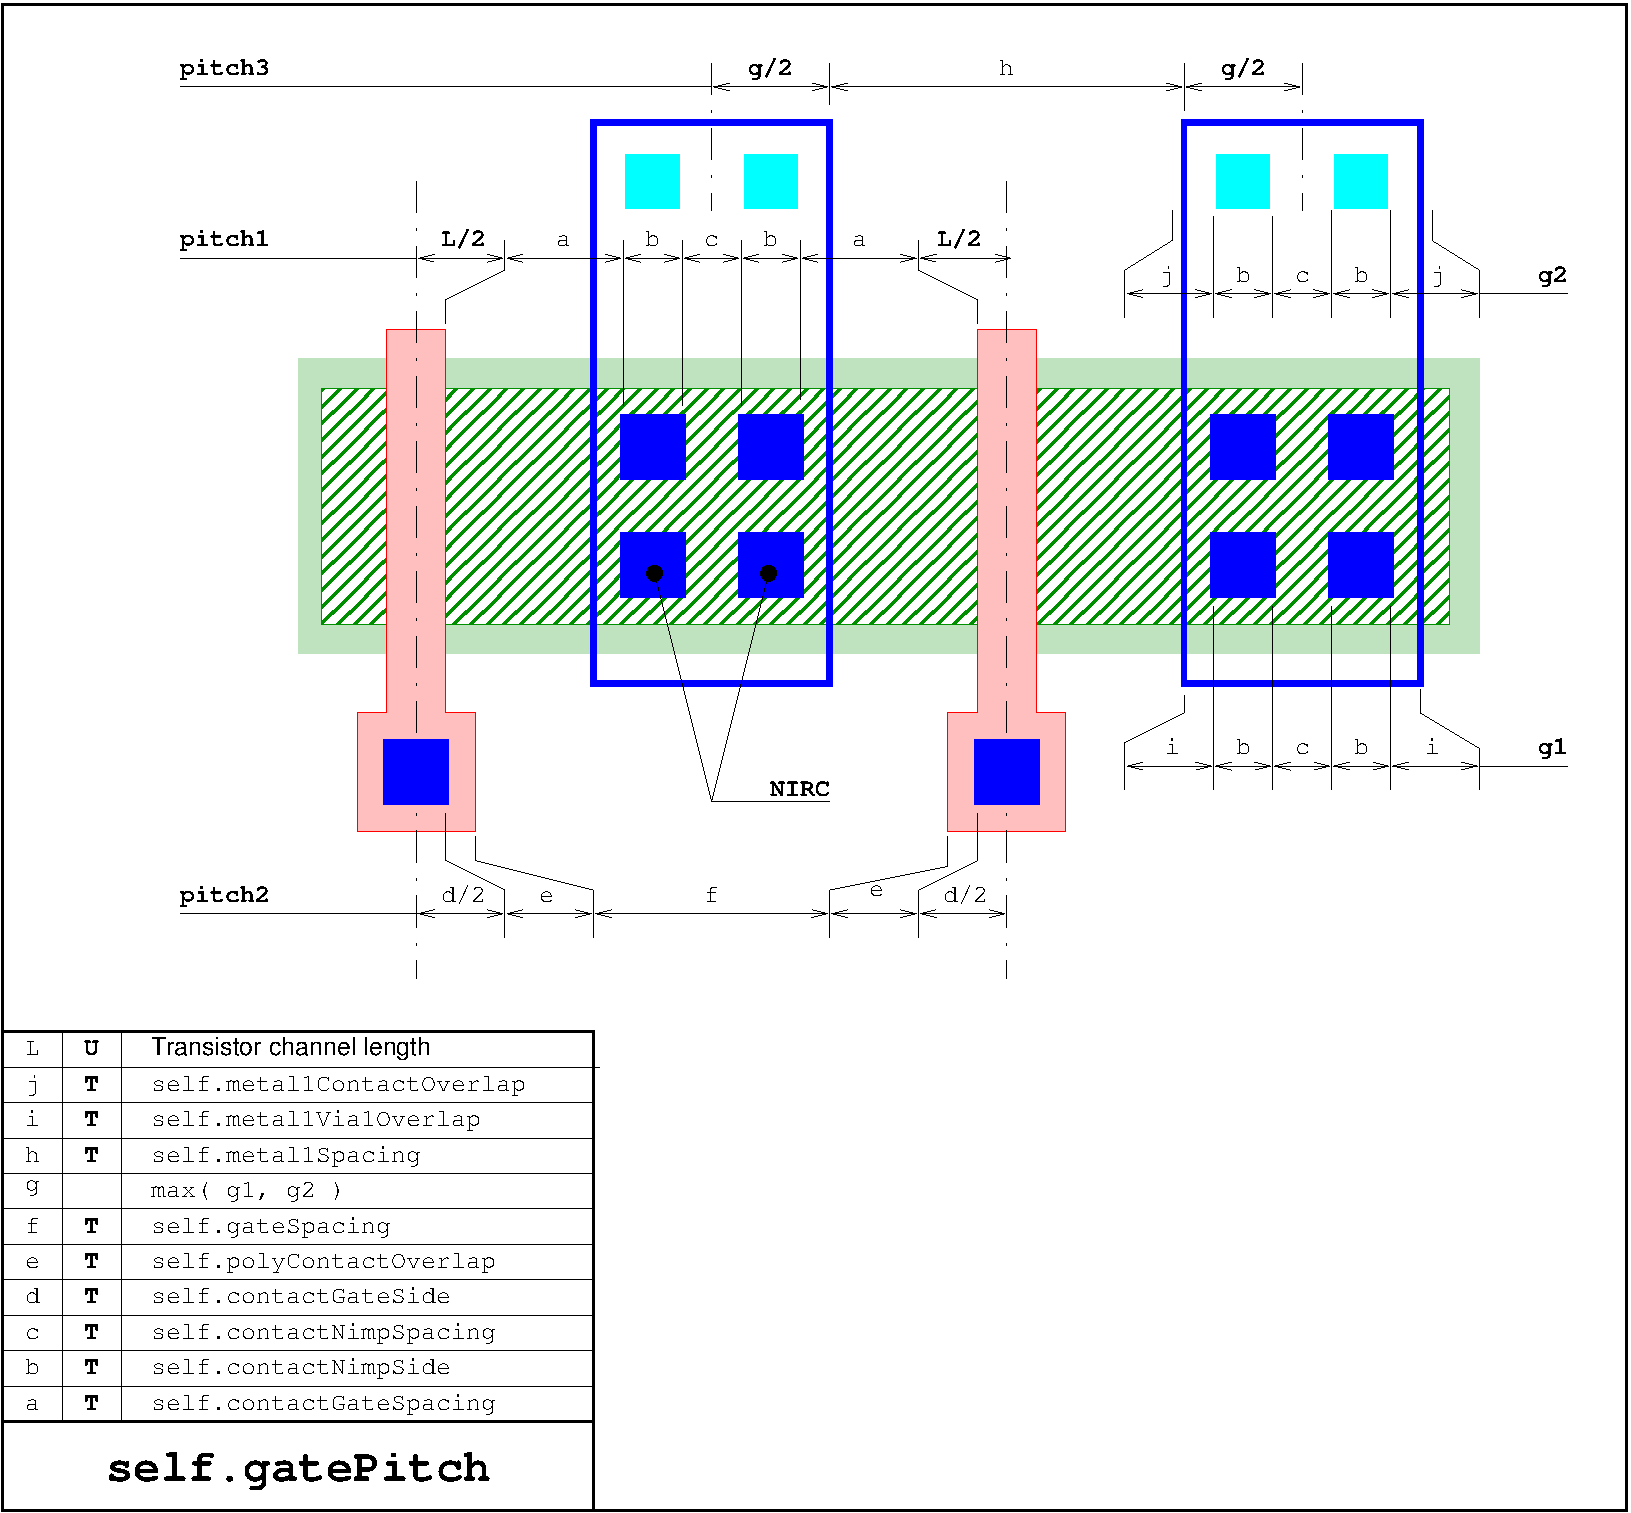
\includegraphics[width=.9\linewidth]{gate-pitch-1}
\caption{Gate Pitch}
\end{DoxyImage}
\hypertarget{classpython_1_1Stack_1_1Stack_secActiveSideWidth}{}\subsubsection{Active Side Width}\label{classpython_1_1Stack_1_1Stack_secActiveSideWidth}

\begin{DoxyItemize}
\item {\ttfamily self.\-active\-Side\-Width} \-: the distance between the axis of the last transistor gate (on the left or right) and the edge of the active area ({\itshape not} the diffusion area).
\end{DoxyItemize}

 
\begin{DoxyImage}
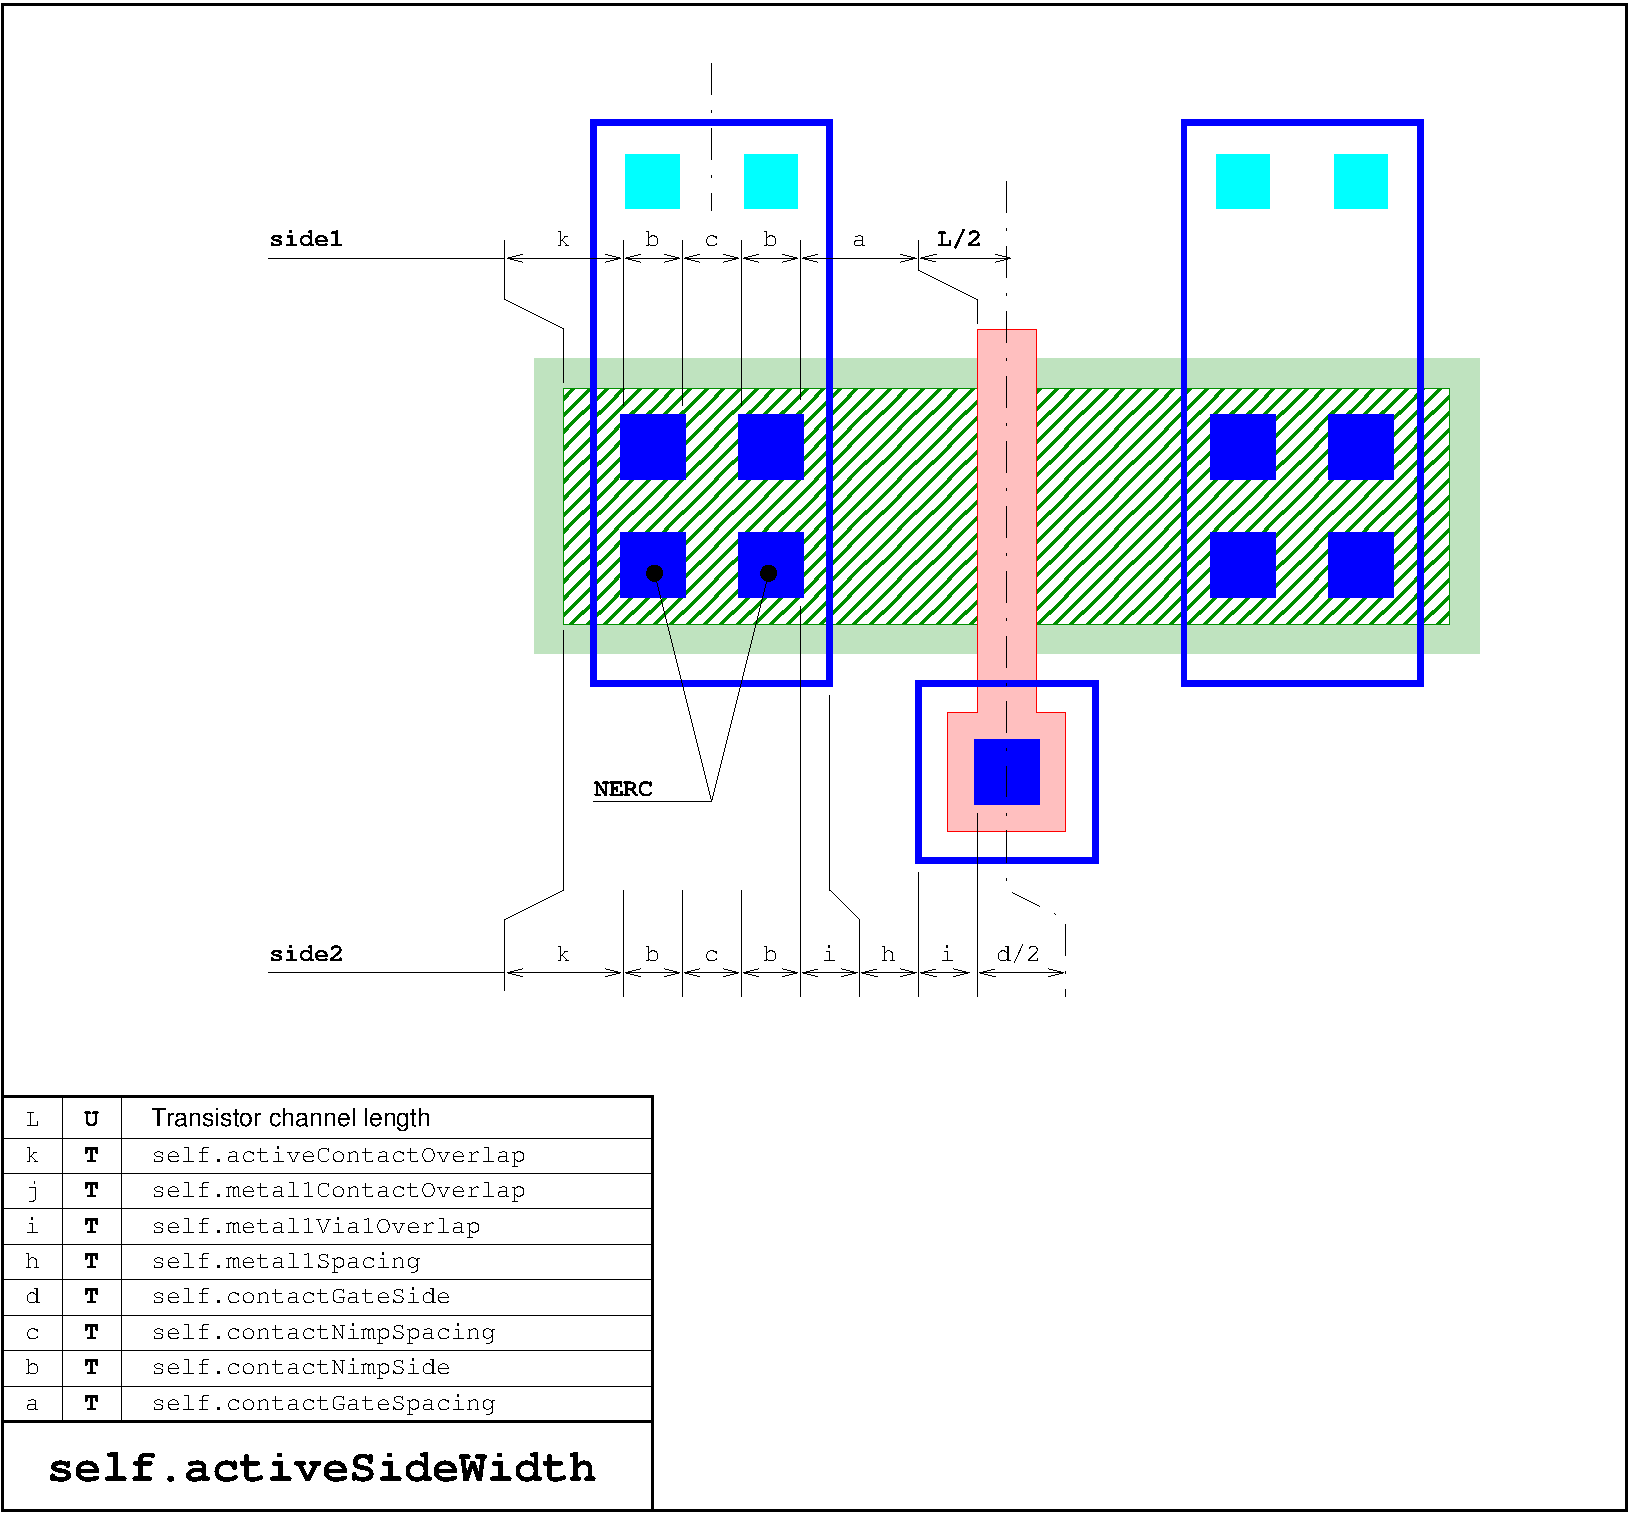
\includegraphics[width=.9\linewidth]{active-side-width-1}
\caption{Active Side Width}
\end{DoxyImage}
\hypertarget{classpython_1_1Stack_1_1Stack_secHTrackDistance}{}\subsubsection{H-\/\-Track Distance}\label{classpython_1_1Stack_1_1Stack_secHTrackDistance}

\begin{DoxyItemize}
\item {\ttfamily self.\-h\-Track\-Distance} \-: the minimal distance between either the top or bottom edge of the active area and the {\itshape axis} of the first track.
\end{DoxyItemize}

 
\begin{DoxyImage}
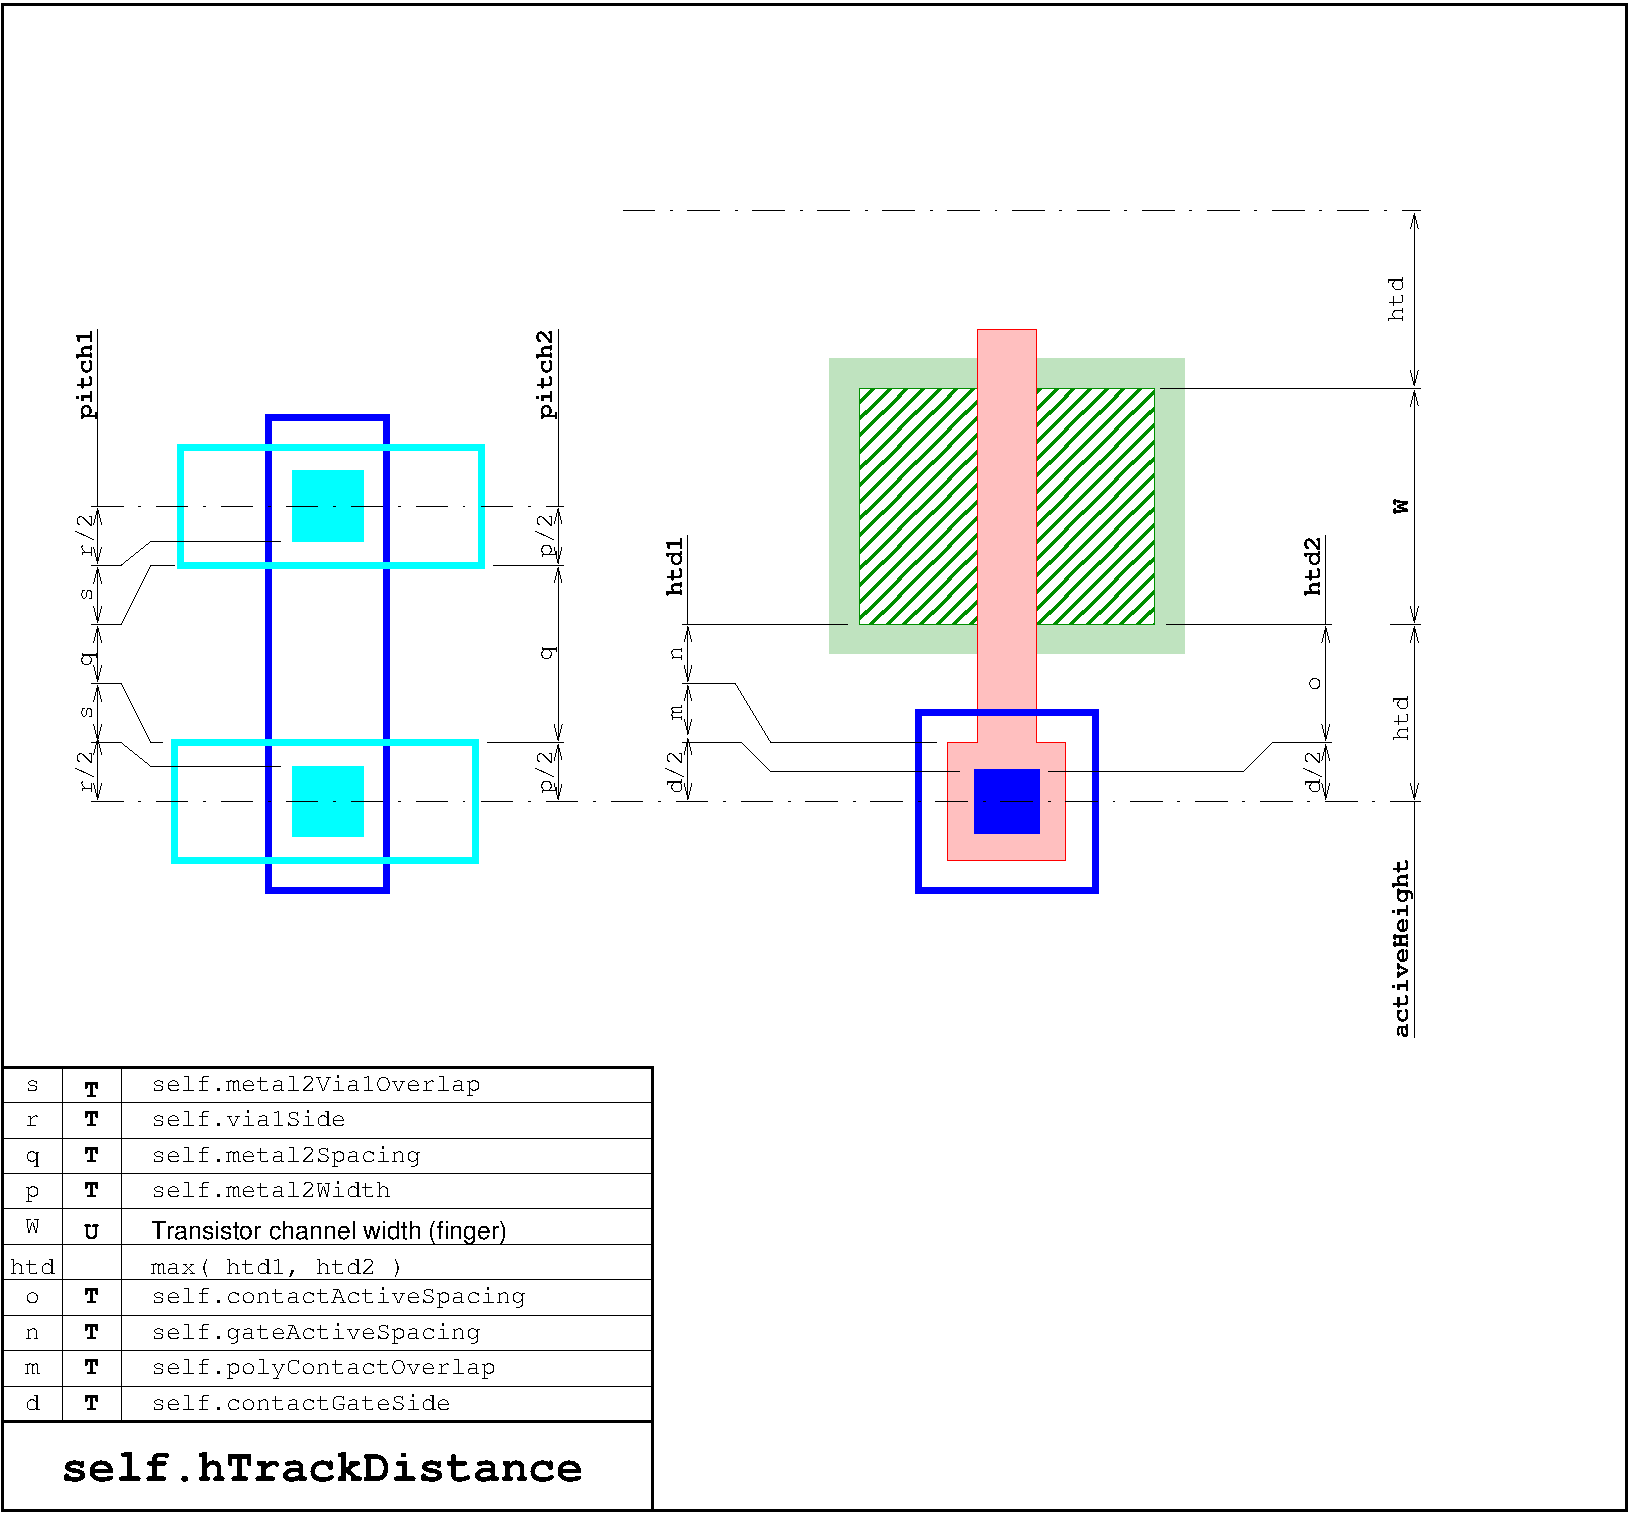
\includegraphics[width=.9\linewidth]{htrack-distance-1}
\caption{H-\/\-Track distance}
\end{DoxyImage}
\hypertarget{classpython_1_1Stack_1_1Stack_secOverallVariables}{}\subsubsection{Bounding\-Box \& Overall Variables}\label{classpython_1_1Stack_1_1Stack_secOverallVariables}

\begin{DoxyItemize}
\item {\ttfamily self.\-xpitches} \-: the number of vertical track pitches needed to fully enclose the active area.
\item {\ttfamily self.\-ypitches} \-: the number of horizontal track pitches needed to fully enclose the active area.
\item {\ttfamily self.\-active\-Offset\-X} \& {\ttfamily self.\-active\-Offset\-Y} \-: the offsets of the active area from the bottom left corner of the abutment box.
\item {\ttfamily self.\-diffusion\-Width} \& {\ttfamily self.\-diffusion\-Height} are the minimun dimensions required to fit the active area.
\item {\ttfamily self.\-top\-Tracks\-Nb()} \-: the number of tracks at the top of the stack.
\item {\ttfamily self.\-bot\-Tracks\-Nb()} \-: the number of tracks at the bottom of the stack.
\end{DoxyItemize}

 
\begin{DoxyImage}
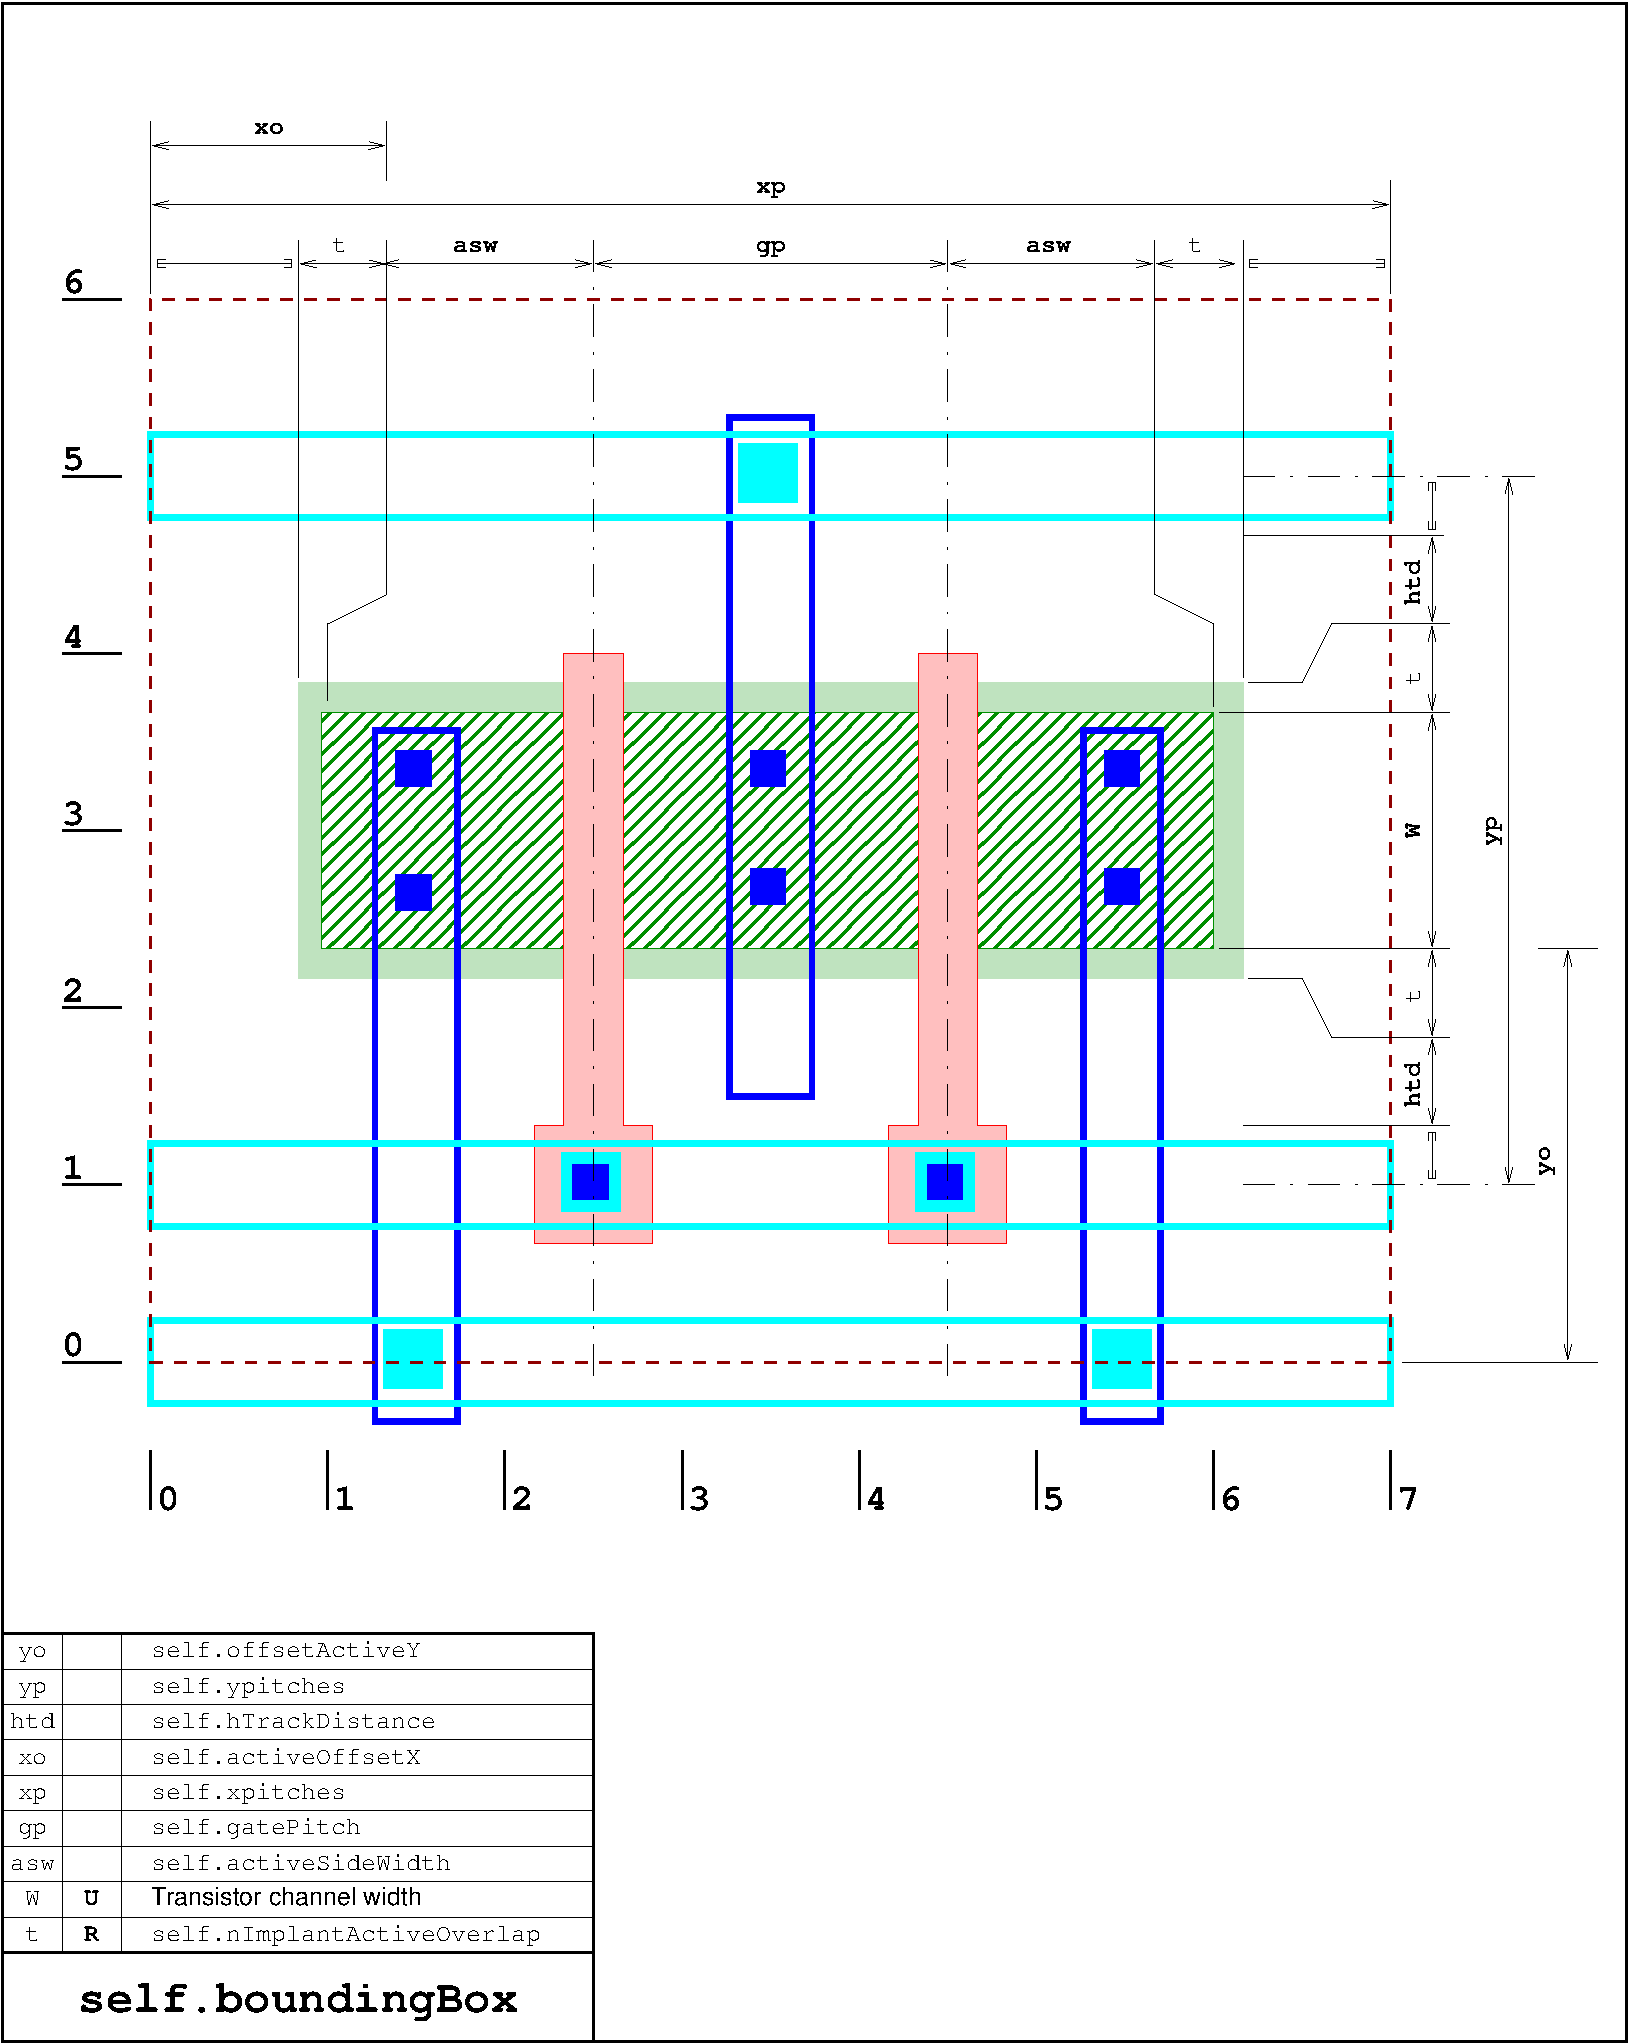
\includegraphics[width=.9\linewidth]{stack-layout-3}
\caption{General Stack Layout}
\end{DoxyImage}
\hypertarget{classpython_1_1Stack_1_1Stack_secWiringSpecs}{}\subsection{Wiring Specifications}\label{classpython_1_1Stack_1_1Stack_secWiringSpecs}
\hyperlink{classpython_1_1Stack_1_1Stack}{Stack} routing is done through vertical {\ttfamily metal1} wires coming from the gates and diffusions areas and {\ttfamily metal2} horizontal wires that can be either above or below the active area. {\ttfamily metal2} wires (or track) goes through the whole stack and are assigned to one net only. A net will have at least one track above or below and may have both.

The connections to the diffusions areas and gates of the various fingers are specified through a list. The stack is made of a regular alternation of diffusions and gates. The list tells, for each one starting from the left, to which net and track they are connected. For a stack of $NFs$ transistor fingers, the must wiring specification must contains $ 3 + (NFs-1) \times 2$ elements. The list is given through one {\itshape string} with each elements separated by one or more whitespace. The syntax for {\itshape one} element is detailed \hyperlink{classpython_1_1Stack_1_1Stack_secAtomicWiring}{Atomic Wiring Specification}.

{\bfseries Track numbering scheme}

Tracks above (top) the active area and below (bottom) each have their own numbering. In both case, the count start {\itshape from} the active area. This, the top tracks will be numbered by increasing Y and the bottom tracks by {\itshape decreasing} Y.

{\bfseries Track/\-Net assignement}

The track/net assignement is deduced from the atomic wiring specifications. It also allows to compute the total number of tracks needed above and below the active area.

 
\begin{DoxyImage}
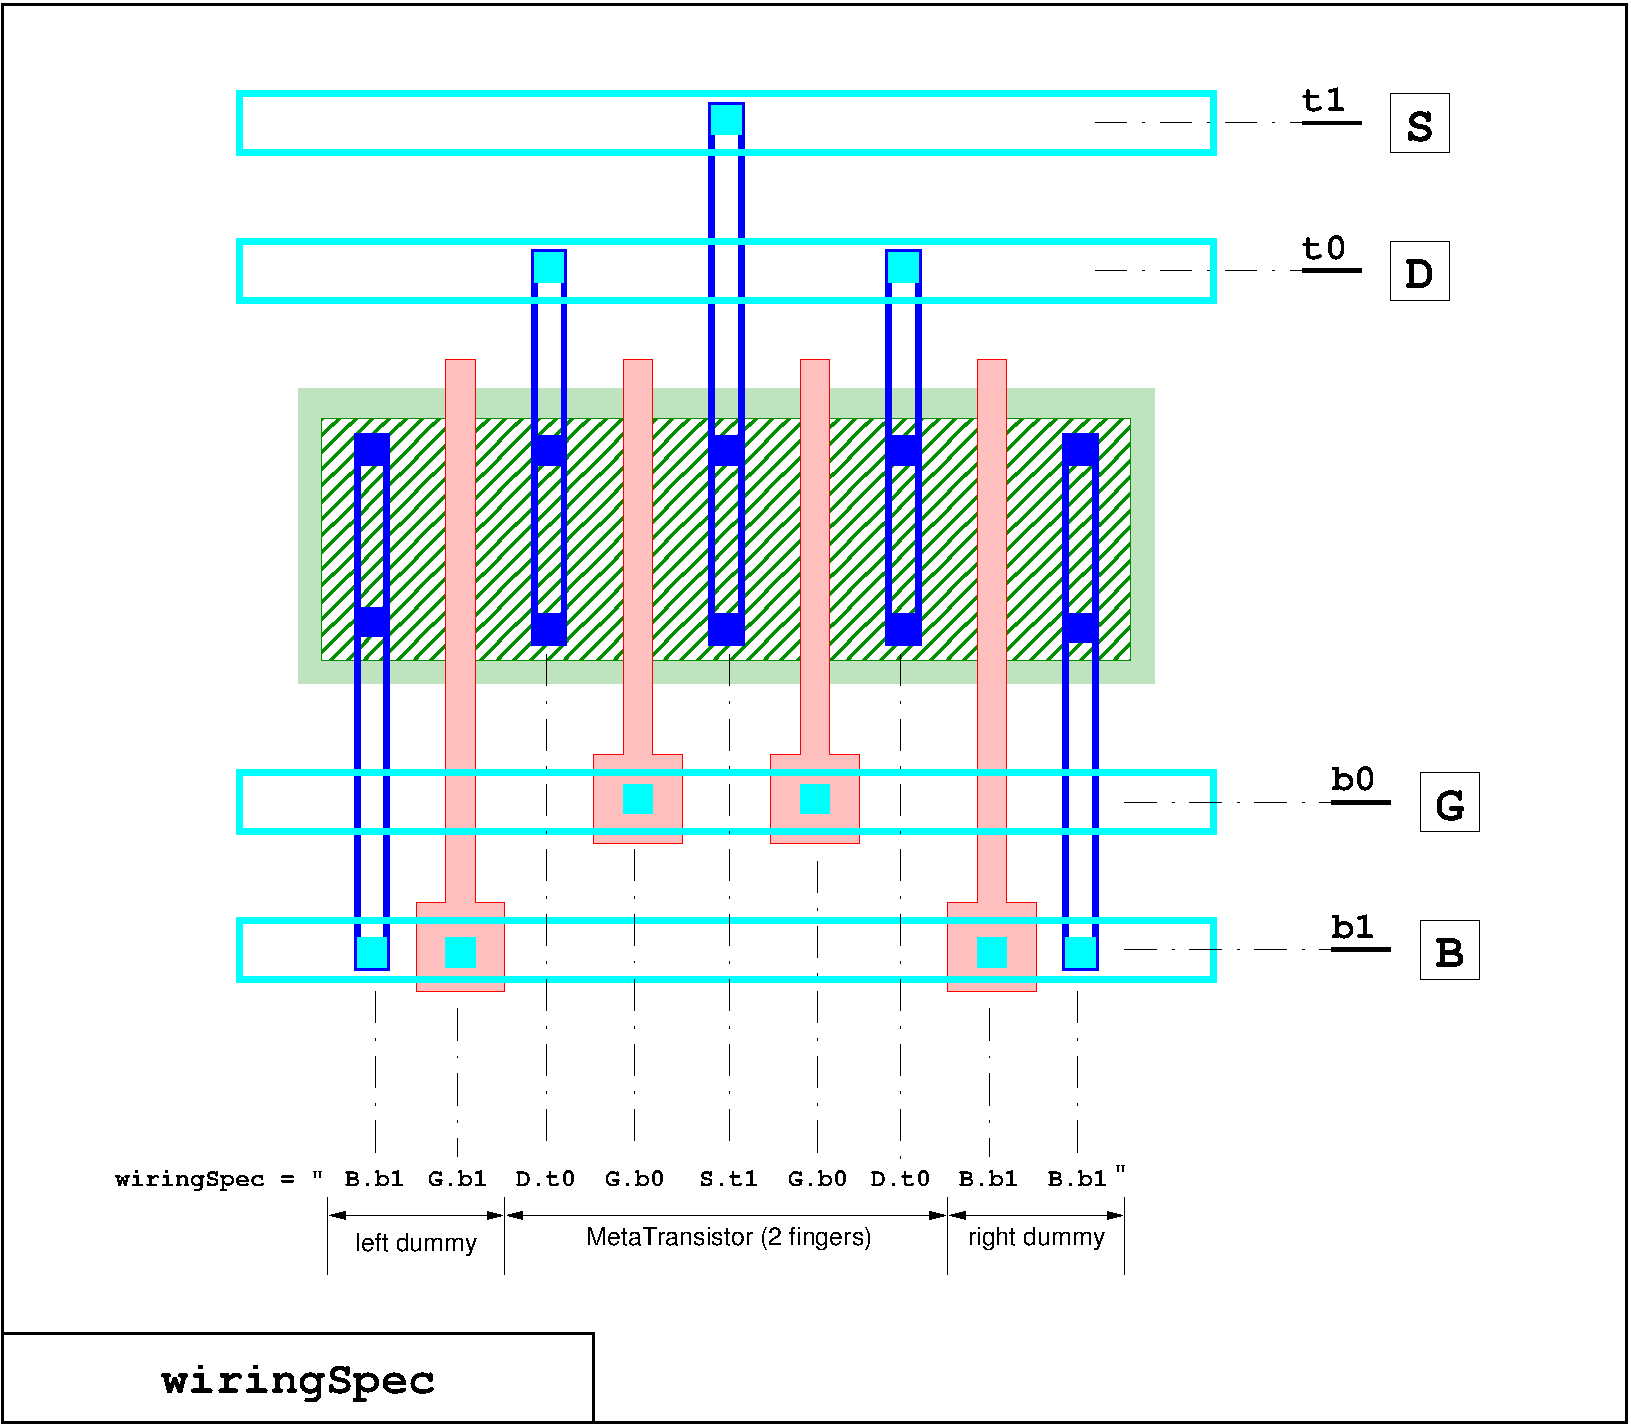
\includegraphics[width=.9\linewidth]{wiring-spec-2}
\caption{Wiring Specification}
\end{DoxyImage}
\hypertarget{classpython_1_1Stack_1_1Stack_secAtomicWiring}{}\subsubsection{Atomic Wiring Specification}\label{classpython_1_1Stack_1_1Stack_secAtomicWiring}
An atomic wiring specification has the same syntax for either diffusions or gates. It {\itshape must} not comprise any whitespaces. it is made of the following parts\-:
\begin{DoxyItemize}
\item The net name to connect to.
\item Whether the track is above the active area ({\ttfamily \char`\"{}t\char`\"{}}) or below ({\ttfamily \char`\"{}b\char`\"{}}). The special case ({\ttfamily \char`\"{}z\char`\"{}}) means that this element must be left unconnected (is such case possible?).
\item The number of the track.
\end{DoxyItemize}

 
\begin{DoxyImage}
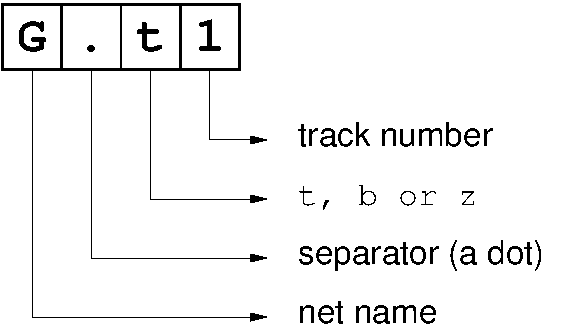
\includegraphics[width=.4\linewidth]{wiring-spec-1}
\caption{Atomic Wiring Specification}
\end{DoxyImage}
\hypertarget{classpython_1_1Stack_1_1Stack_secStackImplDetails}{}\subsection{Stack Implementation Details}\label{classpython_1_1Stack_1_1Stack_secStackImplDetails}
The {\ttfamily \-\_\-\-\_\-setattr\-\_\-\-\_\-()} and {\ttfamily \-\_\-\-\_\-getattr\-\_\-\-\_\-} functions have been redefined so that the technological values (rules) can be accessed has normal attributes of the \hyperlink{classpython_1_1Stack_1_1Stack}{Stack} class, in addition to the regular ones. 

\subsection{Constructor \& Destructor Documentation}
\hypertarget{classpython_1_1Stack_1_1Stack_ac775ee34451fdfa742b318538164070e}{\index{python\-::\-Stack\-::\-Stack@{python\-::\-Stack\-::\-Stack}!\-\_\-\-\_\-init\-\_\-\-\_\-@{\-\_\-\-\_\-init\-\_\-\-\_\-}}
\index{\-\_\-\-\_\-init\-\_\-\-\_\-@{\-\_\-\-\_\-init\-\_\-\-\_\-}!python::Stack::Stack@{python\-::\-Stack\-::\-Stack}}
\subsubsection[{\-\_\-\-\_\-init\-\_\-\-\_\-}]{\setlength{\rightskip}{0pt plus 5cm}def \-\_\-\-\_\-init\-\_\-\-\_\- (
\begin{DoxyParamCaption}
\item[{}]{self, }
\item[{}]{device, }
\item[{}]{N\-E\-R\-C, }
\item[{}]{N\-I\-R\-C}
\end{DoxyParamCaption}
)}}\label{classpython_1_1Stack_1_1Stack_ac775ee34451fdfa742b318538164070e}


{\bfseries \mbox{[}A\-P\-I\mbox{]}} Constructor 

param rules The physical rule set. 
\begin{DoxyParams}{Parameters}
{\em device} & The {\bf Hurricane} A\-M\-S device into which the layout will be drawn. \\
\hline
{\em N\-E\-R\-C} & Number of contact rows in external (first \& last) diffusion connectors. \\
\hline
{\em N\-I\-R\-C} & Number of contact rows in middle diffusion connectors. param w The {\bfseries width} of every transistor of the stack (aka {\itshape fingers}). param L The {\bfseries length} of every transistor. param N\-Fs The total number of fingers (dummies includeds). param N\-Ds The number of dummies to put on each side of the stack. \\
\hline
\end{DoxyParams}


References Stack.\-b\-Implant\-Layer, Stack.\-bot\-Tracks, Stack.\-bot\-W\-Tracks, Stack.\-bulk\-Net, Stack.\-bulks, Stack.\-device, Stack.\-dimensioned, Bulk.\-flags, Stack.\-flags, Stack.\-is\-Nmos(), Stack.\-L, Stack.\-meta\-Tnb(), Stack.\-meta\-Transistors, Stack.\-N\-Ds, Stack.\-N\-E\-R\-C, Stack.\-N\-Fs, Stack.\-N\-I\-R\-C, Stack.\-t\-Implant\-Layer, Stack.\-top\-Tracks, Stack.\-top\-W\-Tracks, Stack.\-w, Stack.\-well\-Layer, and Stack.\-wirings.



\subsection{Member Function Documentation}
\hypertarget{classpython_1_1Stack_1_1Stack_ad7f0300aaad3ad8b2de70ae6c106c102}{\index{python\-::\-Stack\-::\-Stack@{python\-::\-Stack\-::\-Stack}!set\-Wirings@{set\-Wirings}}
\index{set\-Wirings@{set\-Wirings}!python::Stack::Stack@{python\-::\-Stack\-::\-Stack}}
\subsubsection[{set\-Wirings}]{\setlength{\rightskip}{0pt plus 5cm}def set\-Wirings (
\begin{DoxyParamCaption}
\item[{}]{self, }
\item[{}]{wiring\-Spec}
\end{DoxyParamCaption}
)}}\label{classpython_1_1Stack_1_1Stack_ad7f0300aaad3ad8b2de70ae6c106c102}


{\bfseries \mbox{[}A\-P\-I\mbox{]}} Set the \hyperlink{classpython_1_1Stack_1_1Stack}{Stack} wiring specification. 


\begin{DoxyParams}{Parameters}
{\em wiring\-Spec} & A string defining the connections for the gates and diffusion areas.\\
\hline
\end{DoxyParams}
For a comprehensive explanation of the wiring specification, refers to \hyperlink{classpython_1_1Stack_1_1Stack_secWiringSpecs}{Wiring Specifications} . 

References Stack.\-bot\-Tracks, Stack.\-bot\-Tracks\-Nb(), Stack.\-bot\-W\-Tracks, Stack.\-bulk\-Net, Stack.\-compute\-Dimensions(), Stack.\-device, Stack.\-dimensioned, Stack.\-e\-Diff\-Metal1\-Width, Bulk.\-flags, Stack.\-flags, Stack.\-gate\-Pitch, Stack.\-get\-Bot\-Track\-Y(), Stack.\-get\-Horizontal\-Width(), Stack.\-hor\-Pitch, Stack.\-L, Stack.\-metal1\-To\-Gate, Stack.\-meta\-Transistors, Stack.\-side\-Active\-Width, Stack.\-top\-Tracks, Stack.\-top\-Tracks\-Nb(), Stack.\-top\-W\-Tracks, Stack.\-wirings, and Stack.\-ypitches.

\hypertarget{classpython_1_1Stack_1_1Stack_a20b46b43488cc58c302b123a89299d85}{\index{python\-::\-Stack\-::\-Stack@{python\-::\-Stack\-::\-Stack}!compute\-Dimensions@{compute\-Dimensions}}
\index{compute\-Dimensions@{compute\-Dimensions}!python::Stack::Stack@{python\-::\-Stack\-::\-Stack}}
\subsubsection[{compute\-Dimensions}]{\setlength{\rightskip}{0pt plus 5cm}def compute\-Dimensions (
\begin{DoxyParamCaption}
\item[{}]{self}
\end{DoxyParamCaption}
)}}\label{classpython_1_1Stack_1_1Stack_a20b46b43488cc58c302b123a89299d85}


{\bfseries \mbox{[}internal\mbox{]}} Compute \hyperlink{classpython_1_1Stack_1_1Stack}{Stack} dimensions from the technological rules. 

{\bfseries Internal function.} Perform the computation of\-:
\begin{DoxyItemize}
\item {\ttfamily self.\-metal1\-Pitch} 
\item {\ttfamily self.\-min\-Width\-\_\-metal1} 
\item {\ttfamily self.\-metal2\-Pitch} 
\item {\ttfamily self.\-min\-Width\-\_\-metal2} 
\item {\ttfamily self.\-gate\-Pitch} 
\item {\ttfamily self.\-side\-Active\-Width} 
\item {\ttfamily self.\-h\-Track\-Distance} 
\item {\ttfamily self.\-xpitches} 
\item {\ttfamily self.\-ypitches} 
\item {\ttfamily self.\-active\-Offset\-X} 
\item {\ttfamily self.\-active\-Offset\-Y} 
\item {\ttfamily self.\-bounding\-Box} 
\end{DoxyItemize}

References Stack.\-active\-Box, Stack.\-active\-Offset\-X, Stack.\-active\-Offset\-Y, Stack.\-bb\-Height, Stack.\-bb\-Width, Stack.\-bot\-W\-Tracks, Stack.\-bounding\-Box, Stack.\-bulks, Stack.\-bulk\-Width, Stack.\-compute\-Layout\-Parasitics(), Stack.\-compute\-Stress\-Effect(), Stack.\-contact\-Diff\-Pitch, Stack.\-contact\-Diff\-Side, Stack.\-D\-G\-G, Stack.\-D\-G\-I, Stack.\-dimensioned, Stack.\-D\-M\-C\-G, Stack.\-D\-M\-C\-G\-T, Stack.\-D\-M\-C\-I, Stack.\-e\-Diff\-Metal1\-Width, Bulk.\-flags, Stack.\-flags, Stack.\-gate\-Pitch, Stack.\-gate\-Via1\-Pitch, Stack.\-get\-Bot\-Track\-Y(), Stack.\-get\-Horizontal\-Width(), Stack.\-get\-Last\-Top\-Track\-Y(), Stack.\-hor\-Pitch, Stack.\-h\-Track\-Distance, Stack.\-i\-Diff\-Metal1\-Width, Stack.\-is\-V\-H, Stack.\-L, Stack.\-metal1\-To\-Gate, Stack.\-metal2\-Pitch, Stack.\-metal2\-Techno\-Pitch, Stack.\-metal3\-Pitch, Stack.\-N\-E\-R\-C, Stack.\-N\-Fs, Stack.\-N\-I\-R\-C, Stack.\-side\-Active\-Width, Stack.\-tracks\-Nb\-Pitch(), Stack.\-v\-Bulk\-Distance, Stack.\-ver\-Pitch, Stack.\-w, Stack.\-wire1\-Width, Stack.\-wire2\-Width, Stack.\-wire3\-Width, Stack.\-wirings, Stack.\-xpitches, and Stack.\-ypitches.



Referenced by Capacitor\-Unit.\-create(), Stack.\-do\-Layout(), Rout\-Matched\-Capacitor.\-route(), and Stack.\-set\-Wirings().

\hypertarget{classpython_1_1Stack_1_1Stack_affc52c42a8c72dc1125ddce55647a6f9}{\index{python\-::\-Stack\-::\-Stack@{python\-::\-Stack\-::\-Stack}!do\-Layout@{do\-Layout}}
\index{do\-Layout@{do\-Layout}!python::Stack::Stack@{python\-::\-Stack\-::\-Stack}}
\subsubsection[{do\-Layout}]{\setlength{\rightskip}{0pt plus 5cm}def do\-Layout (
\begin{DoxyParamCaption}
\item[{}]{self, }
\item[{}]{bb\-Mode}
\end{DoxyParamCaption}
)}}\label{classpython_1_1Stack_1_1Stack_affc52c42a8c72dc1125ddce55647a6f9}


{\bfseries \mbox{[}A\-P\-I\mbox{]}} Draw the complete layout. 

Draw the commplete layout of the \hyperlink{classpython_1_1Stack_1_1Stack}{Stack}. 

References Stack.\-active\-Offset\-X, Stack.\-active\-Offset\-Y, Stack.\-bb\-Width, Stack.\-bot\-Tracks, Stack.\-bot\-W\-Tracks, Stack.\-bounding\-Box, Stack.\-bulk\-Net, Stack.\-bulks, Stack.\-bulk\-Width, Stack.\-compute\-Dimensions(), Stack.\-contact\-Diff\-Pitch, Stack.\-device, Stack.\-D\-G\-G, Stack.\-D\-G\-I, Stack.\-D\-M\-C\-G, Stack.\-D\-M\-C\-G\-T, Stack.\-D\-M\-C\-I, Stack.\-draw\-Active(), Stack.\-draw\-Gate(), Stack.\-draw\-Source\-Drain(), Stack.\-draw\-Well(), Stack.\-e\-Diff\-Metal1\-Width, Bulk.\-flags, Stack.\-flags, Stack.\-gate\-Pitch, Stack.\-gate\-Via1\-Pitch, Stack.\-get\-Bot\-Track\-Y(), Stack.\-get\-Horizontal\-Axis(), Stack.\-get\-Horizontal\-Width(), Stack.\-get\-Top\-Track\-Y(), Stack.\-get\-Wiring\-Width(), Stack.\-hor\-Pitch, Stack.\-i\-Diff\-Metal1\-Width, Stack.\-is\-Bot\-Track(), Stack.\-is\-V\-H, Stack.\-L, Stack.\-metal1\-To\-Gate, Stack.\-N\-E\-R\-C, Stack.\-N\-Fs, Stack.\-N\-I\-R\-C, Stack.\-side\-Active\-Width, Stack.\-t\-Implant\-Layer, Stack.\-top\-Tracks, Stack.\-top\-W\-Tracks, Stack.\-w, Stack.\-well\-Layer, Stack.\-wire1\-Width, Stack.\-wire2\-Width, Stack.\-wire3\-Width, and Stack.\-wirings.



The documentation for this class was generated from the following file\-:\begin{DoxyCompactItemize}
\item 
Stack.\-py\end{DoxyCompactItemize}

%--- End generated contents ---

% Index
\backmatter
\newpage
\phantomsection
\clearemptydoublepage
\addcontentsline{toc}{chapter}{Index}
\printindex

\end{document}
